\usepackage{color}
\usepackage{amsmath}
\usepackage{graphicx}
%%
\title{
\jtitle{内発的動機付けと対照学習の改良によるスパースな報酬環境における探索効率向上}
\etitle{Enhancing Exploration Efficiency in Sparse Reward Environments through Refined Intrinsic Motivation and Contrastive Learning}
}
%%英文は以下を使用
%\title{Style file for manuscripts of JSAI 20XX}

\jaddress{ 相良博喜,九州大学 数理学府,福岡県福岡市西区元岡744,sagara.hiroki.043@s.kyushu-u.ac.jp }

\author{%
\jname{相良博喜\first}
\ename{Hiroki Sagara}
\and
\jname{屋藤翔麻\second}
\ename{Shoma Yato}
\and
\jname{草場壽一\third}
\ename{Shuichi Kusaba}
%\and
%Given-name Surname\third{}%%英文は左を使用
}

\affiliate{
\jname{\first{}九州大学}
\ename{Kyushu University}
\and
\jname{\second{}東京工芸大学}
\ename{Tokyo Polytechnic University}
\and
\jname{\third{}東京大学}
\ename{University of Tokyo}
}

%%
%\Vol{28}        %% <-- 28th(変更しないでください)
%\session{0A0-00}%% <-- 講演ID(必須)

\begin{abstract}
We propose a method to enhance exploration efficiency in reinforcement learning environments with sparse rewards by improving intrinsic motivation and contrastive learning. Intrinsic motivation is used to guide agents to novel states by providing internal rewards based on prediction errors. However, existing methods such as Random Network Distillation (RND) suffer from declining intrinsic rewards over time, leading to limited exploration in later stages. To address this, we introduce two modifications: (1) adjusting intrinsic rewards when episodes terminate due to agent failure, and (2) enhancing contrastive learning by treating temporally adjacent frames as positive examples. These modifications improve novelty detection and encourage consistent exploration. Experiments in sparse-reward environments such as Climber demonstrate significant improvements, with our method achieving external rewards in half the training steps compared to baseline models. Our approach maintains high intrinsic reward peaks throughout training, paving the way for more effective exploration in challenging environments.
\end{abstract}

%\setcounter{page}{1}
\def\Style{``jsaiac.sty''}
\def\BibTeX{{\rm B\kern-.05em{\sc i\kern-.025em b}\kern-.08em%
 T\kern-.1667em\lower.7ex\hbox{E}\kern-.125emX}}
\def\JBibTeX{\leavevmode\lower .6ex\hbox{J}\kern-0.15em\BibTeX}
\def\LaTeXe{\LaTeX\kern.15em2$_{\textstyle\varepsilon}$}

\begin{document}
\maketitle

\section{研究背景・目的}
強化学習(Reinforcement Learning; RL)の分野は近年目覚ましい進歩を遂げている。多様なタスクへの対応、意思決定から複雑なゲームの習得に至るまで、その応用範囲を広げてきた。これらの進展は、計算能力の向上と機械学習手法、特にディープラーニングのブレークスルーによって推進されてきた。しかし、報酬信号が希薄な環境における効率的な探索は依然として大きな課題である。このような環境では、エージェントが複雑な状態空間を効率的にナビゲートし、限られたフィードバックから学習する能力が求められる。この問題に対する有望な解決策として、内発的動機(Intrinsic Motivation; IM)\cite{IM}が挙げられる。IMは、新奇性や驚きなどの内部信号を活用して探索を導き、学習効率を高める。

この分野で注目すべき研究の一つが、Random Network Distillation(RND)\cite{RND}である。RNDは、新奇性検出に基づく手法であり、固定されたランダムなターゲットネットワークと予測モデルを用い、予測モデルがターゲットネットワークの出力を模倣しようとする際に生じる誤差を新奇性の指標として用い、エージェントに探索の指標となる内発的報酬を提供する。この手法は報酬が希薄な環境でも効率よく学習することが可能であったが、固定されたターゲットネットワークに依存するため、学習が進むにつれて誤差が少なくなり内発的報酬が消失するという課題がある。

こうした課題を克服するために提案されたのが、Self-supervised Network Distillation(SND)\cite{SND}である。SNDは、ターゲットネットワークを自己教師あり学習によって動的に学習させることで、ターゲットモデルの表現を適応的に進化させ、新奇性検出の精度を向上させる。

本研究では、このSNDフレームワークをさらに改良するために2つの取り組みを行った。最初の取り組みは、内発的動機に基づく行動において、エピソード終了時の挙動を調整するためのηの最適化である。内発的動機に基づく行動は、新たな状態に対して無作為に取り組むため、短期間で敵と衝突するなどしてエピソードが終了してしまい、効率的な学習が妨げられる可能性がある。これに対処するため、高い内発的動機によってエピソードが終了した場合、その内発的動機に基づく報酬にマイナスの補正を加える方法を試みる。

2つ目の取り組みは、内発的動機の学習方法を見直すことである。特に対照学習(Contrastive Learning)を行う際、Noisy TV問題が発生することを考慮した。この問題は、エージェントが一時的な新奇性に過度に引き付けられ、環境の本質的な目標から注意が逸れる現象を指す。既往研究においても、ProcgenベンチマークのPitfallのようなゲームで、NPCの点滅やランダム動作にエージェントの関心が不適切に引きつけられ、報酬を得ることができないという課題があった。他の環境においても、初期状態におけるキャラクターの無作為な前後移動がノイズとして作用し、エージェントの探索効率を妨げる可能性がある。この問題に対処するため、対照学習を行う際に前後フレームを考慮し、連続するフレームを同一の状態として学習させる手法を導入する。

\section{関連研究}
強化学習(Reinforcement Learning; RL)は報酬が希薄な環境での探索効率を向上させるために、多くの手法が研究されている。その中でも、内発的動機付け(Intrinsic Motivation; IM)は、生物学的動機付けを模倣したアプローチとして注目されており、新奇性や予測誤差などの内部的な信号を探索の指針として用いる\cite{RL},\cite{IM}。IMは、「知識ベース」と「能力ベース」の2つの主要なアプローチに分類される\cite{IM2},\cite{IM3}。知識ベースのアプローチは、探索を通じてエージェントが世界の知識を獲得することに焦点を当て、予測誤差を利用する予測ベースの手法、新奇性を指標とするノベルティベースの手法、情報理論的指標を活用する手法に細分化される\cite{UCEIM},\cite{IMS}。能力ベースのアプローチは、エージェントがスキルを習得し環境内での目標達成能力を向上させることを目的としている\cite{CDE}。

内発的動機付けに関する包括的な調査では、これらの手法が探索性能を高める上で有効である一方、それぞれの制約や実装上の課題も指摘されている\cite{IMRL},\cite{IMRL2}。特に、予測ベースの手法として代表的なランダムネットワーク蒸留(Random Network Distillation; RND)は、固定されたターゲットネットワークと予測モデルの出力誤差を新奇性の指標とすることで探索を促進するが、ターゲットネットワークが静的であるため、学習が進むにつれて内発的報酬が減少し、後半の探索が停滞するという問題がある\cite{RND},\cite{IMRL},\cite{IMRL2}。一方、好奇心主導型学習を大規模に検証した研究では、新奇性指標や情報理論的アプローチの有用性が示されている\cite{CSL}。情報理論的アプローチとしては、環境動態モデルの情報ゲインを内発的報酬とする VIME(Variational Information Maximizing Exploration)の例が挙げられる\cite{VIME}。

自己教師あり学習(Self-Supervised Learning)を活用した手法としては、BYOL-Explore や VICReg などがあり、モンテズマの復讐や ProcGen 環境のような高難易度タスクにおいても有効な探索を実現している\cite{BYOL},\cite{SEMRE}。さらに、エージェントが環境を内部モデルとして捉える「世界モデル(World Models)」の概念が近年注目を集めている\cite{WM}\cite{CB}。世界モデルでは、エージェントが環境のダイナミクスを学習し、内部的な予測や計画、さらには潜在表現を用いた目標生成を通じて探索を促進することが可能となる\cite{IMRL},\cite{IMRL2},\cite{LTP},\cite{WDM},\cite{AWMPC},\cite{LLD},\cite{DAG}。こうした世界モデルの枠組みにおいても、内発的動機付けはエージェントが未知の状態を積極的に探索するための強力な駆動力となる。
一方、内発的動機付け手法においては、環境中の純粋なノイズや人間のエージェントにとって有益でない情報(いわゆる "Noisy TV")が過剰に興味を引いてしまう問題が指摘されている\cite{IM},\cite{CB}。この問題に対処するためには、タスク達成や学習効率の観点からノイズを制御する仕組みや報酬設計が必要であるとされる。強化学習アルゴリズムとしては、方策勾配法の一種である PPO(Proximal Policy Optimization)が、実装の容易さと安定性から広く利用されており、内発的動機付け手法との組み合わせによりスパース報酬環境でも効果的な学習が期待される\cite{PPO}。

\section{提案手法}
\subsection{SNDの基本的な手法}
SNDは、内発的動機付けを活用し、報酬が希薄な環境における探索効率を向上させる手法である。
具体的には、強化学習における報酬に、内発的報酬\(r^{\text{intr}}\)と外的報酬\(r^{\text{ext}}\)の合成を用いて、新奇性の高い行動へエージェントを誘導する。
\[
 r_t = r^{\text{ext}}_{t} + \eta \cdot r^{\text{intr}}_{t}
\]
ここで、\(\eta\)は内発的報酬の重み付け係数である。
\begin{figure}[t]
   \centering
   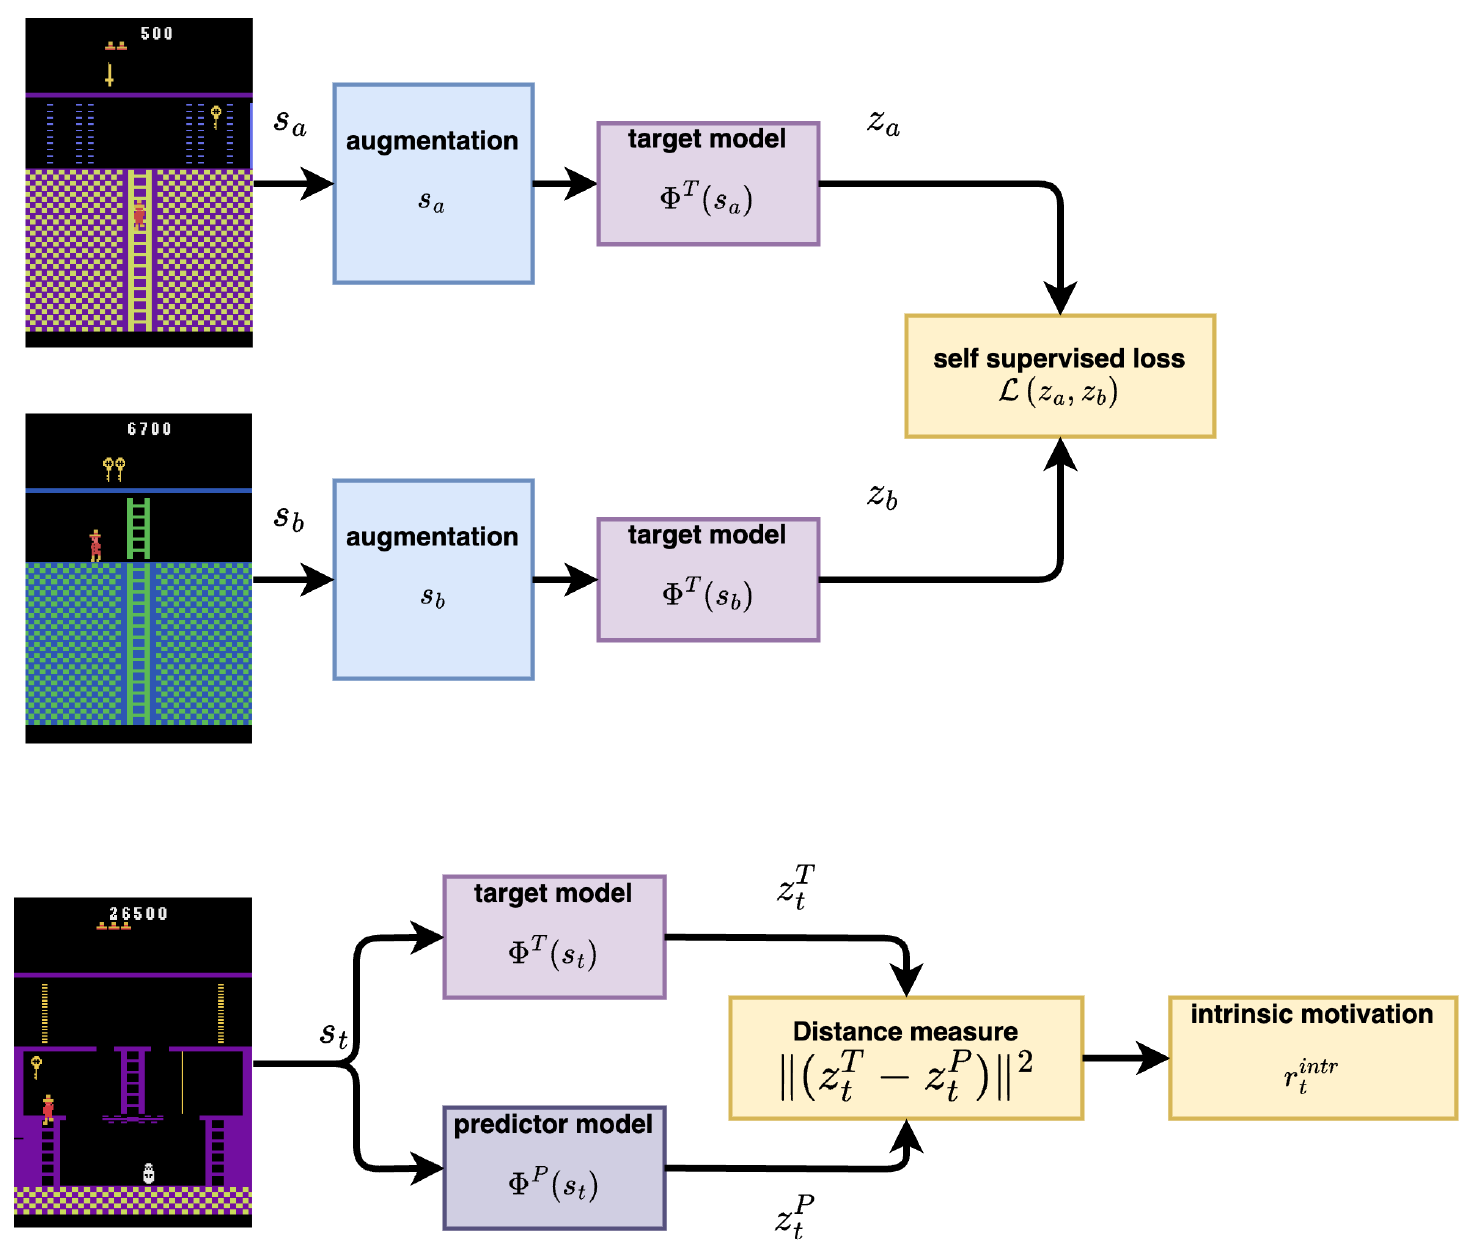
\includegraphics[width=0.5\textwidth]{figure1.eps}
   \caption{自己教師ありネットワーク蒸留(SND)の原理。本手法は2つの主要な部分で構成されている。上図: ターゲットモデルを自己教師あり学習にて適切な特徴ベクトルを学習する。 下図: ターゲットモデルと予測モデルの誤差から内発的報酬を得る。本図は\cite{SND}より転載。}\label{fig1:figure1}
\end{figure}
\begin{figure}[t]
   \centering
   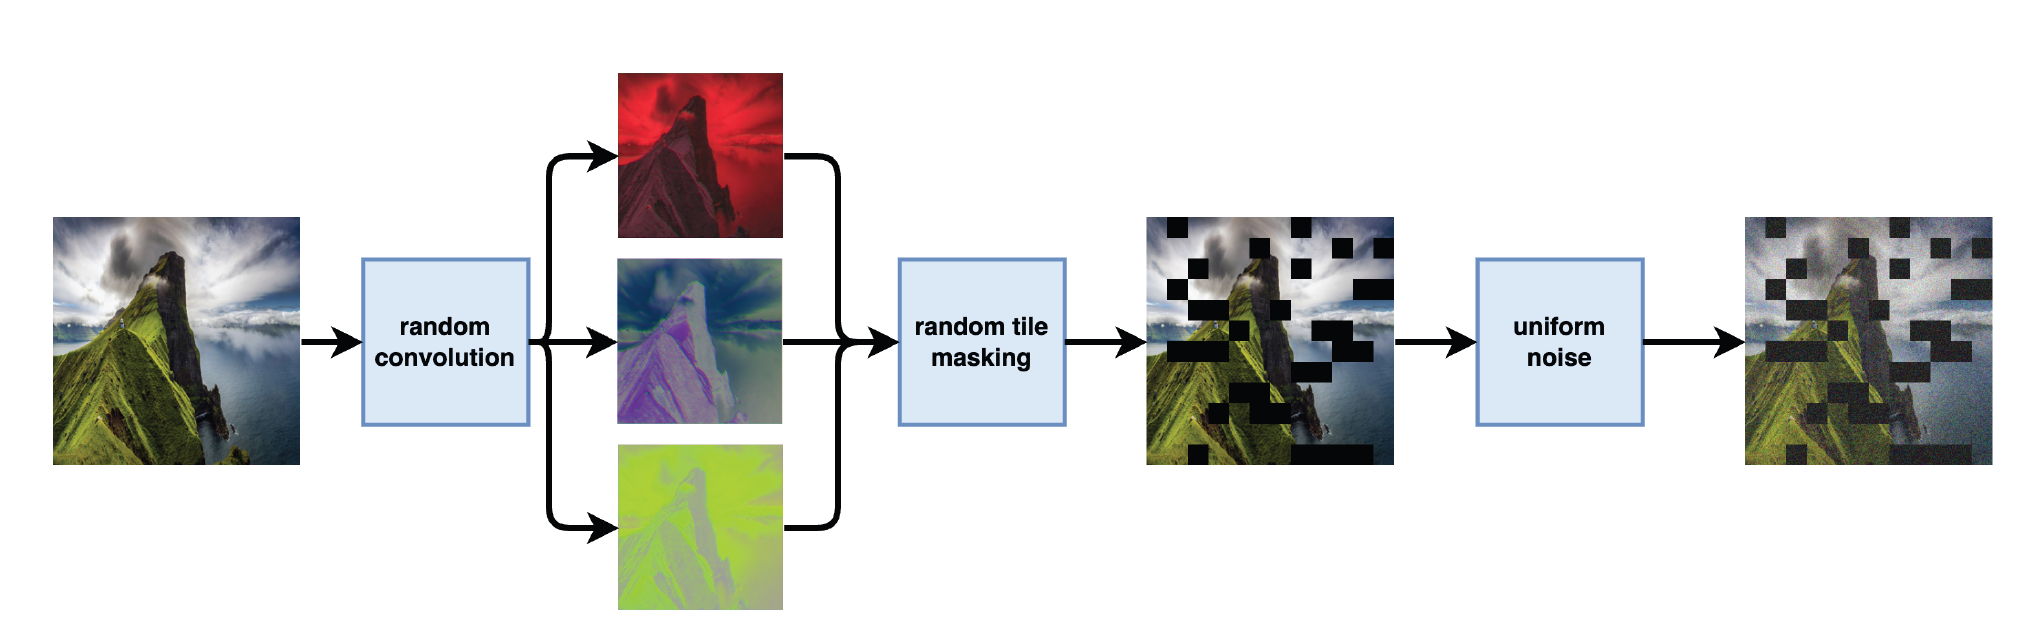
\includegraphics[width=0.5\textwidth]{figure2.eps}
   \caption{SND-Vのデータオーグメンテーション方法 本図は\cite{SND}より転載。}\label{fig2:figure2}
\end{figure}


内発的報酬は、予測モデル\(\Phi_P\)とターゲットモデル\(\Phi_T\)の間の誤差を内発的報酬として利用する[図\ref{fig1:figure1}]。
この誤差は以下の式で定義される:
\[
 r^{\text{intr}}_{t} = \| \Phi_T(s_t) - \Phi_P(s_t) \|_2^2,
\]
ここで、\(s_t\)は現在の状態を表し、\(\|\cdot\|_2^2\)はL2ノルムの2乗を意味する。この誤差は、新奇性を評価する指標として利用され、新しい状態ほど大きな値を取る。
予測モデルは、以下の損失関数で定義される通り、ターゲットモデルの出力を模倣するよう学習が行われる。
\[
 L_P = \frac{1}{N} \sum_{s \in S} \| \Phi_T(s) - \Phi_P(s) \|_2^2,
\]
つまり、RNDのようにターゲットモデルが固定されたアルゴリズムの場合、最終的には内発的報酬が収束してしまい内発的報酬が発生しなくなる。
SNDでは、自己教師あり学習を利用してターゲットモデルを動的に更新し、状態表現の分散性を向上させる。
本研究では既往論文にて提案されているSND-Vというアルゴリズムを用いた。

\subsection{SND-V}
SND-Vは対照学習をベースとした新奇性検出手法である。
類似する状態の特徴を近づけ、異なる状態を分離する損失関数を用いることで、特徴空間を効果的に構築する。
また、状態にノイズを付与することで、ロバストな特徴表現を学習することができる。

SND-Vにおける損失関数の定義は以下の通りである:
\[
 L_T = \sum_{n} (\tau_n - \| Z_n - Z'_n \|_2^2)^2,
\]
ただし、\(\tau_n = 0\)の場合、\(Z_n\)および\(Z'_n\)は同じ状態に対してノイズを付与した状態に対する特徴ベクトルを表す。
\(\tau_n = 1\)の場合、\(Z_n\)および\(Z'_n\)は全く異なる状態、異なるエピソード、異なるステップに対してノイズを付与した状態に対する特徴ベクトルである。

ノイズの付与方法は既往研究と同様に[図\ref{fig2:figure2}]、下記3つのフィルタをp=0.5の確率で適用する。

・ 一様ランダムノイズ:ピクセル値に\([-1, 1]\)の範囲でノイズを追加。

・ ランダムマスキング:画像タイルをランダムにマスクする(タイルサイズは2、4、8、12、16ピクセル)。

・ ランダム畳み込みフィルタ

\subsection{提案する改良手法}
本研究では、SNDの基本的な枠組みに加え、探索効率および報酬取得の向上を目指して以下の2つの改良手法を提案する。

\subsection{改善手法1:エピソード終了時の報酬調整}
 内発的動機に基づく行動は、新たな状態に対して無作為に取り組むため、短期間で敵と衝突するなどしてエピソードが終了してしまい、効率的な学習が妨げられる可能性がある。これに対処するため、高い内発的動機によってエピソードが終了した場合、その内発的動機に基づく報酬にマイナスの補正を加える方法を試みた。
エピソード終了時における新たなルールを導入した。具体的には、エピソード終了時に\(\text{level\_complete} = \text{false}\)かつゲーム終了までのステップ数に到達していない場合、その状態を"死亡"とみなす。この場合、報酬は以下のように定義される:
\[
 r_t = \begin{cases}
 r_{\text{ext}, t} - \eta \cdot r_{\text{intr}, t}, & \text{死亡の場合},\\
 r_{\text{ext}, t} + \eta \cdot r_{\text{intr}, t}, & \text{それ以外の場合}.
\end{cases}
\]
内発的報酬が大きい状況にて死亡が発生した場合、その行動がエージェントの継続的な探索を妨げてしまっていると考えられる。このため、死亡時に内発的報酬にマイナスの補正を加えることで、エージェントがより長期的に探索を行うことができ、効率的な学習が可能となることが期待される。


\subsection{類似状態ペア選択方法の改善}
前章で述べた通り、Noisy TV問題とはエージェントが時系列的なノイズに不適切に関心を持ち、探索が非効率化する現象を指す。

例えば、初期状態におけるキャラクターの無作為な前後移動がノイズとして作用し、エージェントの探索効率を妨げる可能性がある。この問題に対処するため、対照学習を行う際に前後フレームを考慮し、連続するフレームを同一の状態として学習させる手法を導入する。これにより、初期状態でのランダムな動作や視覚的なノイズをエージェントの興味の対象から外し、より本質的な違いに基づく状態に関心を移すことが期待される。
具体的には、SND-Vに下記の改良を加えた。

1. 同一環境およびSTEPが\(-N\)から\(+N\)ステップの範囲内にある\(2N+1\)個の状態からランダムに選択する。

2. 選択した状態にノイズを加え、類似状態ペアを構成する。

3. 非類似状態の選択は既往研究と同様にランダムに行う。

このアプローチでは、既往研究のSND-Vが採用していた完全に同一の状態ペアからノイズを加える方式よりも多様な状態表現を学習できる。特に周期的に変化する状態を同一状態と捉え、無駄な内発的報酬の発生を抑えることが期待される。これにより、状態空間全体でより精度の高い新奇性検出が可能となり、エージェントが短期的なノイズではなく本質的な環境変化に基づいて行動できるようになる。

\section{実験・考察}

\subsection{実験設定}
本研究では、Self-supervised Network Distillation(SND)\cite{SND}の条件設定を引き継ぎ、提案手法の有効性を検証した。具体的には、ProcGenベンチマークのClimber環境において、提案手法を適用し、探索効率および報酬取得の改善を評価した。

\subsection{改善手法1: エピソード終了時の報酬調整}
まず、エピソード終了時の報酬調整の効果を検証した。\ref{fig3:figure3}
\begin{figure}[t]
   \centering
   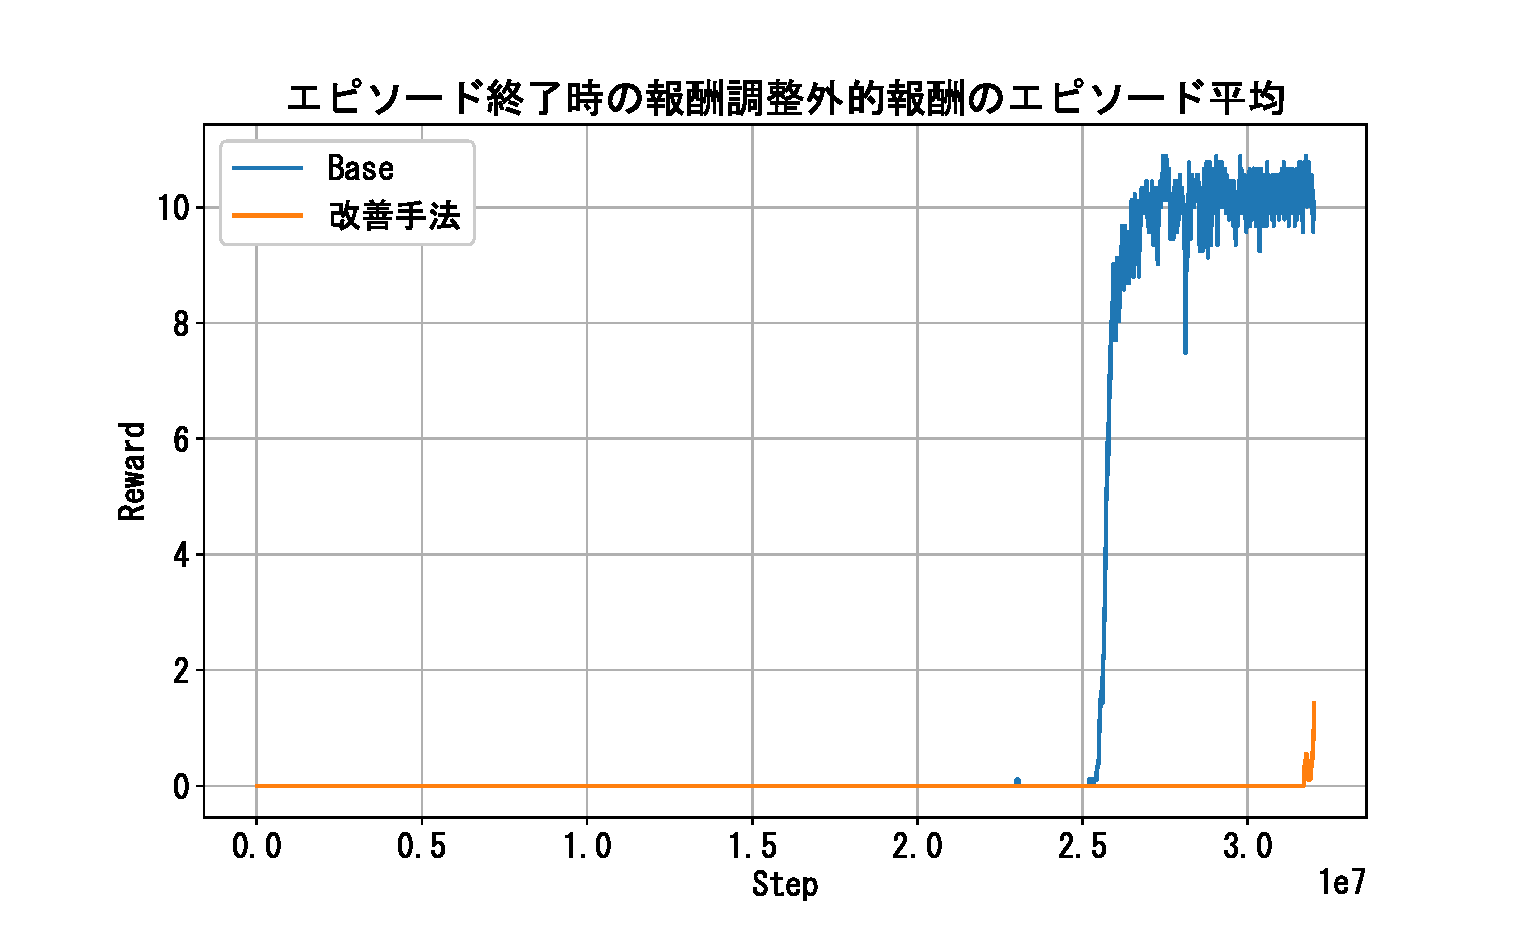
\includegraphics[width=0.5\textwidth]{Method1_Ext.eps}
   \caption{改善手法1: エピソード終了時の報酬調整 外的報酬の推移}\label{fig3:figure3}
\end{figure}
\begin{figure}[t]
   \centering
   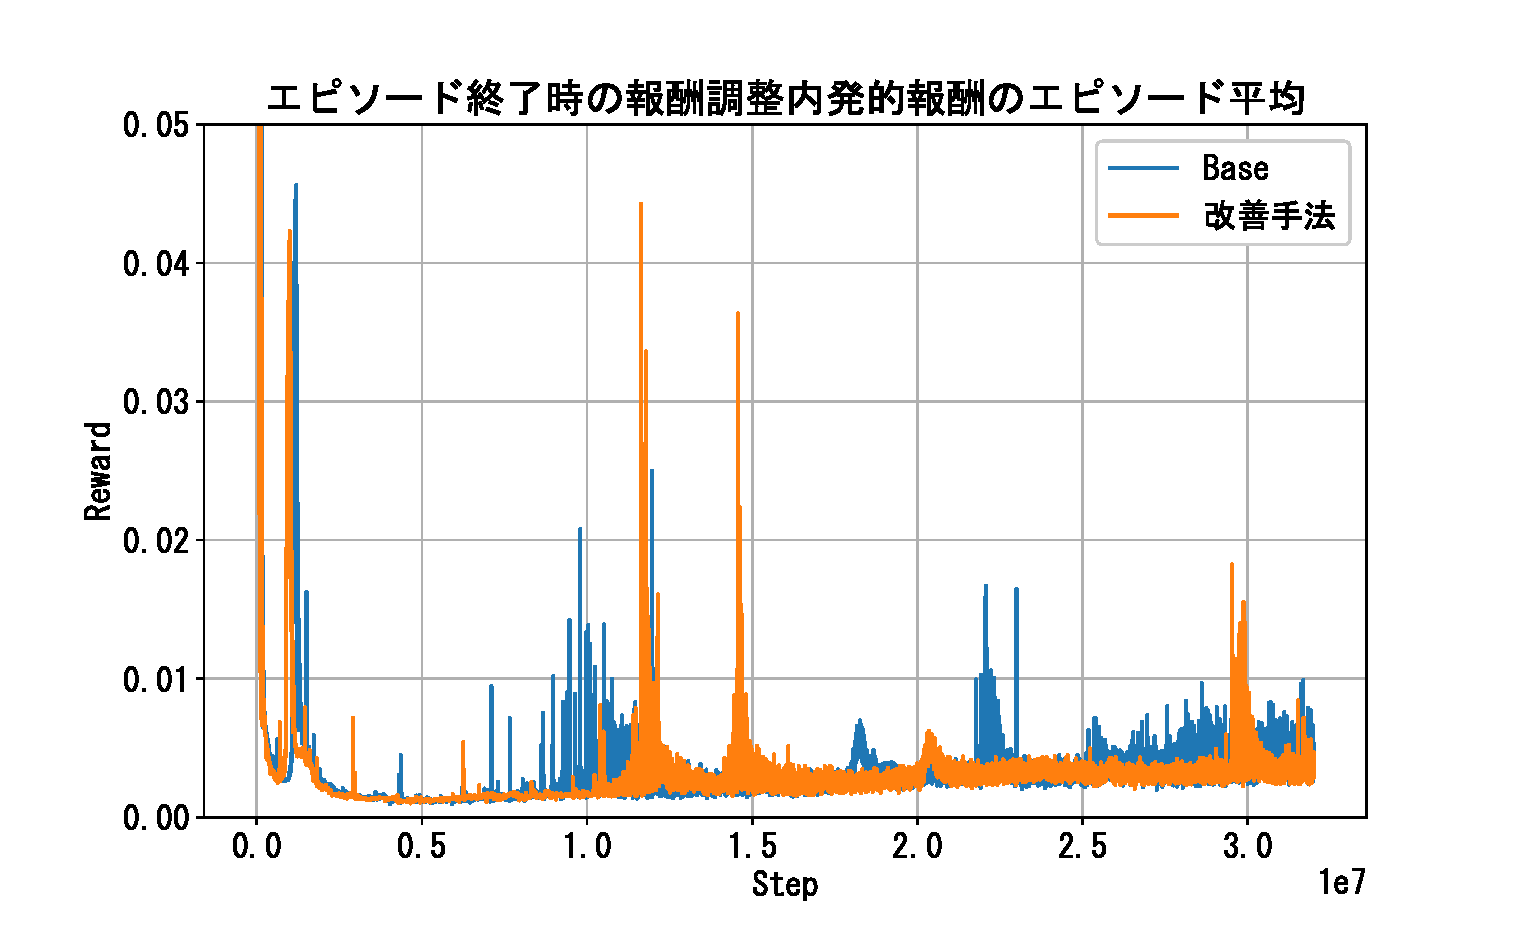
\includegraphics[width=0.5\textwidth]{Method1_Intr.eps}
   \caption{改善手法1: エピソード終了時の報酬調整 内発的報酬の推移}\label{fig4:figure4}
\end{figure}

結果から、提案手法が既往研究のモデルより外部報酬を得るまでの時間が長くなっていることがわかる。
また、内発的報酬に関しても、既往研究のモデルよりもピークの発生回数が少なく、内発的動機による行動が発生していないことがわかる。\ref{fig4:figure4}
このような結果となった原因を分析するため、エピソード終了時までのステップ数を生存時間解析(Kaplan-Meier法)により評価した。
[図\ref{fig7:figure7}]
\begin{figure}[t]
   \centering
   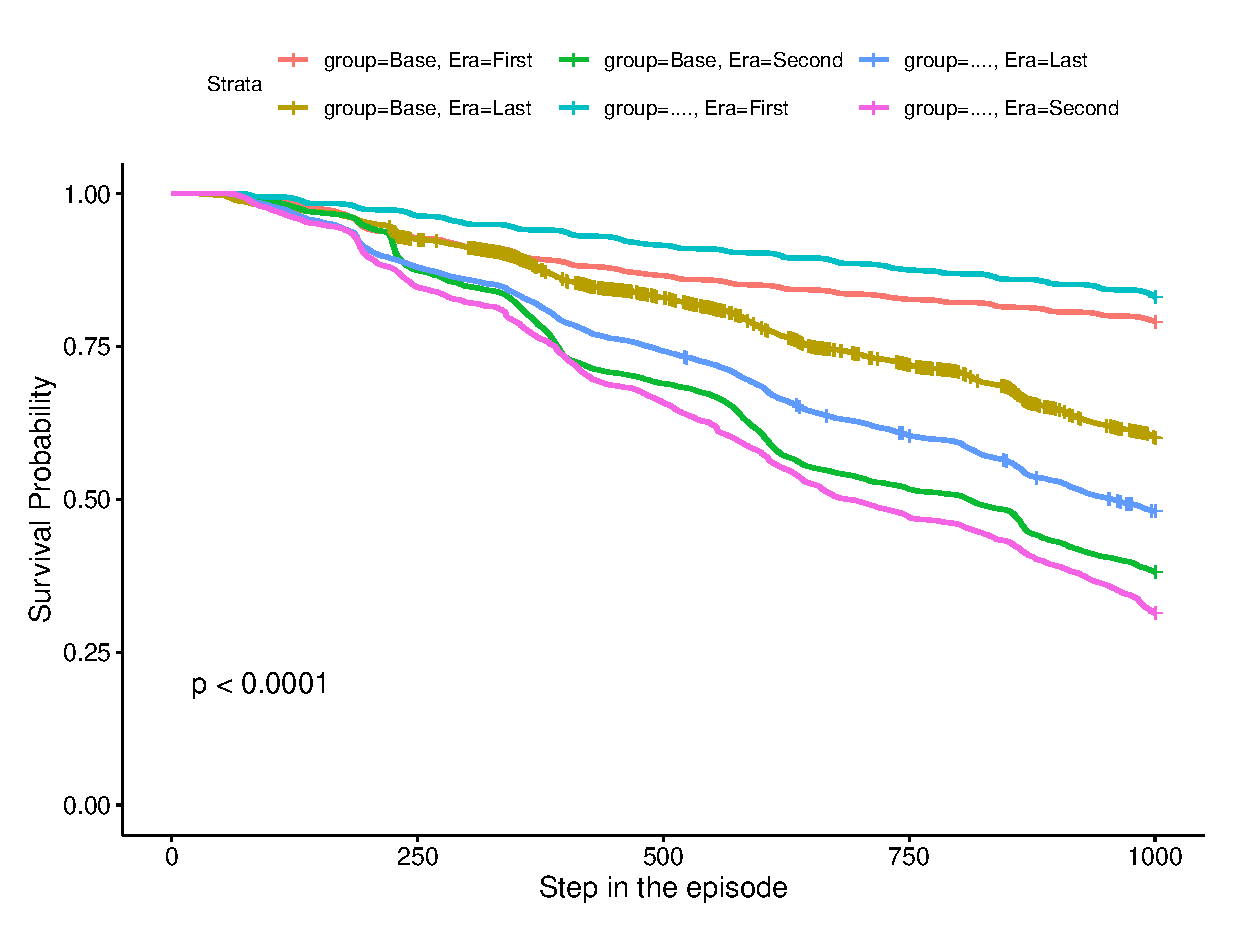
\includegraphics[width=0.5\textwidth]{kaplan_meier_plot.eps}
   \caption{エピソード内でのキャラクター生存期間 Kaplan-meierプロット Base= 既往研究 Method1= 改善手法1 Era:First= 1~1.0e7 Step, Second=1.0e7~2.0e7 Step, Last=2.0e7~ Step}\label{fig7:figure7}
\end{figure}
まだ十分に学習が進んでいない序盤に関しては、提案手法が既往研究のモデルよりも生存時間が長い。しかし、学習が進むにつれて提案手法の生存時間が短くなっていることがわかる。これは、提案手法により序盤の探索が積極的に行われず、中盤以降の学習が遅れていることを示唆していると考えられる。

\subsection{改善手法2: 類似状態ペア選択方法の改善}
次に、類似状態ペア選択方法の改善の効果を検証した。本実験では、ペアの選択範囲はN=1、つまり前後ステップの状態を選択する方法を採用した。
\begin{figure}[h]
   \centering
   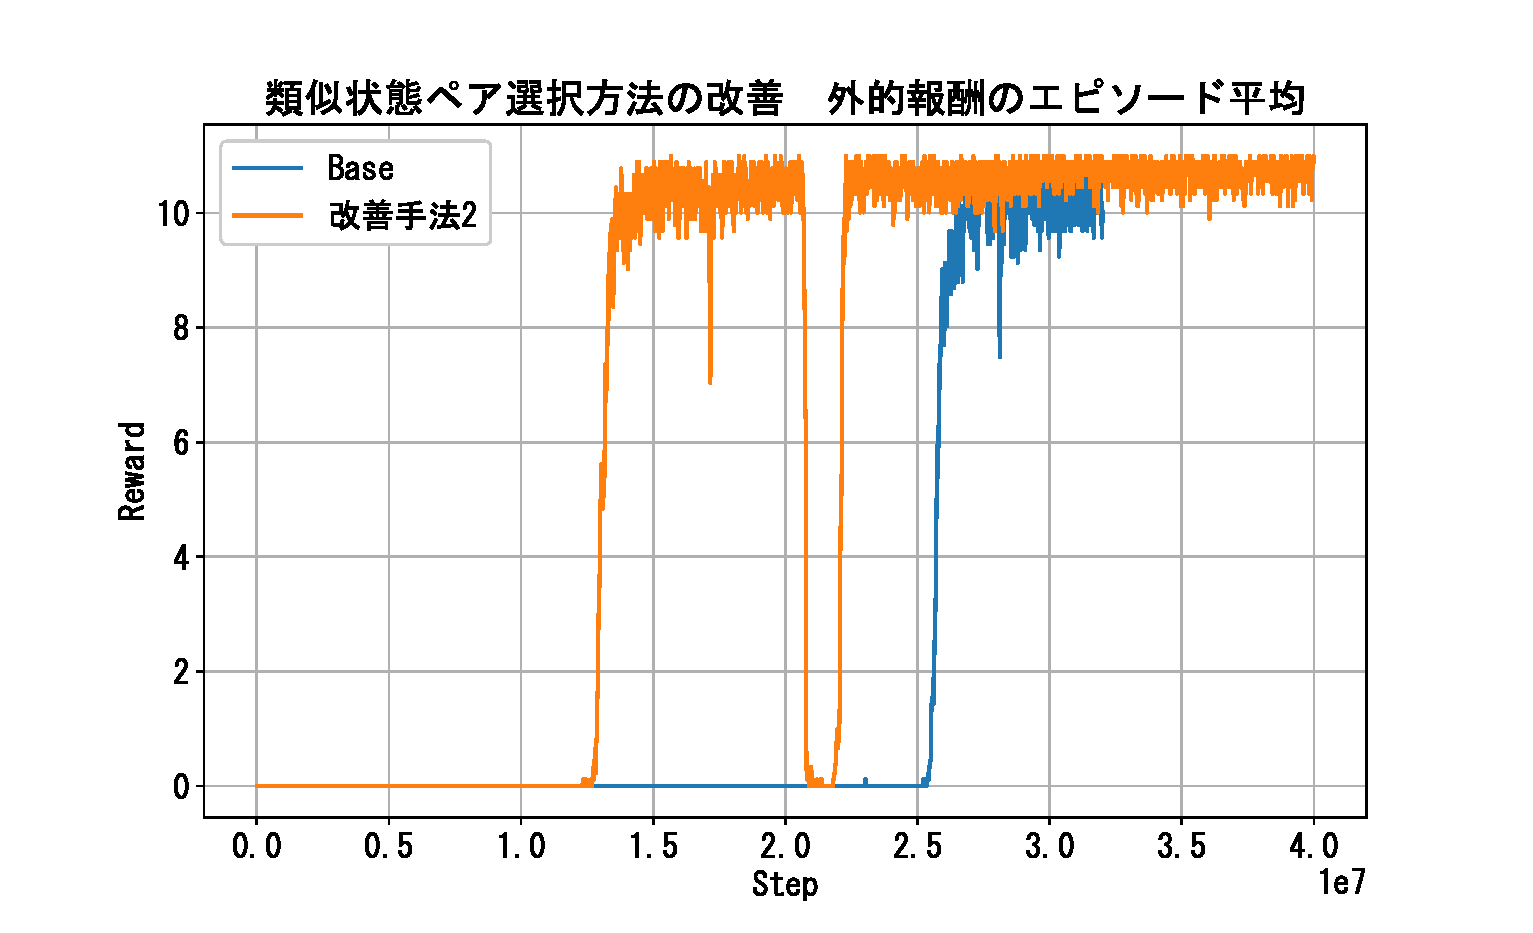
\includegraphics[width=0.5\textwidth]{Method2_Ext.eps}
   \caption{改善手法2: 類似状態ペア選択方法の改善 外的報酬の推移}\label{fig5:figure5}
\end{figure}
\begin{figure}[h]
   \centering
   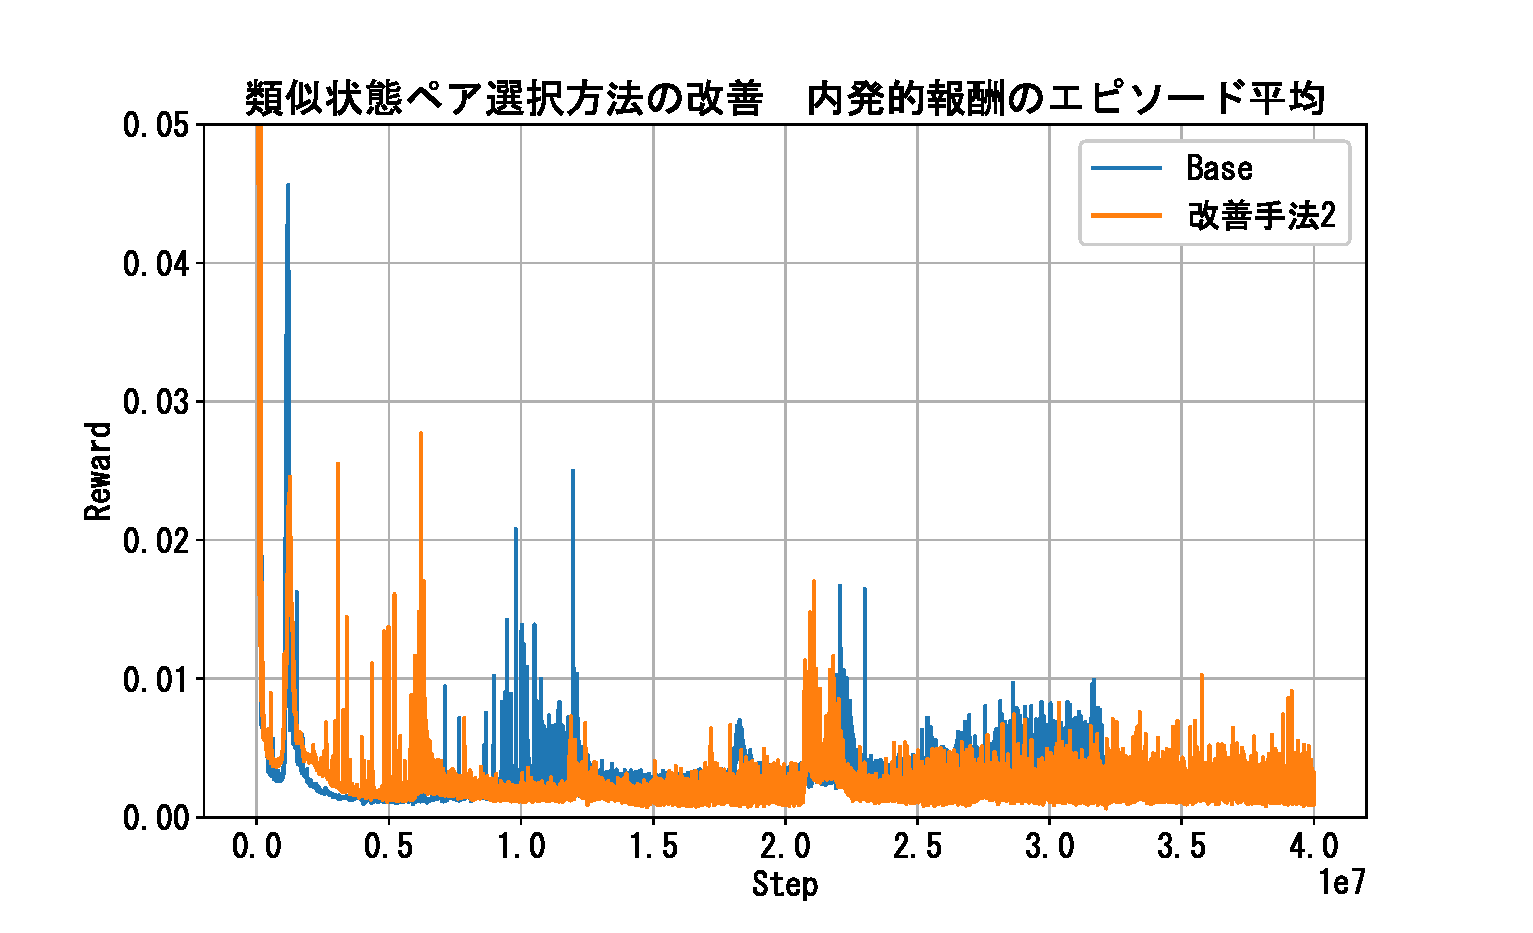
\includegraphics[width=0.5\textwidth]{Method2_Intr.eps}
   \caption{改善手法2: 類似状態ペア選択方法の改善 内発的報酬の推移}\label{fig6:figure6}
\end{figure}
[図\ref{fig5:figure5}]が本手法の外部報酬の推移である。既往研究では、2.6e7ステップで初めて外部報酬を得たが、提案手法では1.3e7ステップ、つまり半分以下のステップ数で外部報酬を獲得していることがわかる。
また、内発的報酬[図\ref{fig6:figure6}]に関しても、違いがある。0.1~0.8e7ステップの間において、既往研究では内発的動機のピークは現れないが、提案手法では内発的動機のピークが現れていることがわかる。

学習序盤で高い内発的動機を得ることができた要因として、エージェントが適切な行動を選択することができず摂動状態に陥ることがあるが、提案手法では大きな状態変化を得ることができ、内発的動機が発生しやすくなっていることが考えられる。これにより学習序盤の探索効率が向上し、外部報酬を得るまでの時間が短くなっていると考えられる。

\section{まとめ}
本研究では、内発的報酬調整と対照学習の改良により、報酬が希薄な環境での探索効率を向上させる手法を提案し、Climberでの実験においてその効果を実証した。
今後は、より難易度の高いゲーム環境(Montezuma's Revenge, Pitfallなど)での検証を進め、提案手法の汎用性を評価する必要がある。

また、将来的な研究の方向性として、外発的報酬のスケーリングパラメータの最適化がある。

時間に基づくスケジューリング: 学習の進行に伴い、内発的動機に基づく探索を減少させることで、探索から活用へのスムーズな移行を実現する。
\[
   \eta(t) = \eta_{\text{init}} \cdot e^{-\alpha t}
\]
このアプローチは学習初期の探索強化と後半の目標指向行動を両立できる。

報酬に基づくスケジューリング:外部報酬の頻度や大きさに応じた適応的な探索と活用の調整を可能にする。
\[
\eta = \frac{1}{1 + \beta \cdot r_{\text{ext}}}
\]
報酬がスパースな環境や動的に変化する環境において、より柔軟な学習を実現する。
これらの手法は、探索と活用のバランスを最適化し、効率的な学習を実現することが期待される。

\begin{thebibliography}{99}
   \bibitem[1]{RL}
   Sutton, R. S., Barto, A. G.
   Reinforcement Learning: An Introduction.
   MIT Press (1998).
   \bibitem[2]{IM}
   P. -Y. Oudeyer, F. Kaplan and V. V. Hafner.
   Intrinsic Motivation Systems for Autonomous Mental Development.
   IEEE Transactions on Evolutionary Computation, vol. 11, no. 2, pp. 265-286 (2007).
   \bibitem[3]{RND}
   Yuri Burda and Harrison Edwards and Amos Storkey and Oleg Klimov.
   Exploration by random network distillation.
   International Conference on Learning Representations (2019).
   \bibitem[4]{SND}
   Matej Pecháč, Michal Chovanec, Igor Farkaš.
   Self-supervised network distillation: An effective approach to exploration in sparse reward environments.
   Neurocomputing.
   Volume 599 (2024).
   \bibitem[5]{IM2}
   Ryan, R. M., Deci, E. L.
   Intrinsic and extrinsic motivations: Classic definitions and new directions.
   Contemporary Educational Psychology, 25(1), 54-67 (2000).
   \bibitem[6]{IM3}
   Deci, E. L., Ryan, R. M.
   Intrinsic Motivation and Self-Determination in Human Behavior.
   Springer Science and Business Media (1985).

   \bibitem[7]{UCEIM}
   Bellemare, M. G., Srinivasan, S., Ostrovski, G., Schaul, T., Saxton, D., Munos, R.
   Unifying Count-Based Exploration and Intrinsic Motivation.
   Advances in Neural Information Processing Systems, vol. 29 (2016).

   \bibitem[8]{IMS}
   Aubret, A., Matignon, L., Hassas, S.
   A Survey on Intrinsic Motivation in Reinforcement Learning.
   arXiv:1908.06976 (2019).

   \bibitem[9]{CDE}
   Pathak, D., Agrawal, P., Efros, A. A., Darrell, T.
   Curiosity-Driven Exploration by Self-Supervised Prediction.
   In Proceedings of the IEEE Conference on Computer Vision and Pattern Recognition (CVPR) (2017).

   \bibitem[10]{IMRL}
   Yuan, M.
   Intrinsically-Motivated Reinforcement Learning: A Brief Introduction.
   arXiv:2203.02298 (2022).

   \bibitem[11]{CSL}
   Burda, Y., Edwards, H., Pathak, D., Storkey, A., Darrell, T., Efros, A. A.
   Large-Scale Study of Curiosity-Driven Learning.
   arXiv:1808.04355 (2018).

   \bibitem[12]{VIME}
   Houthooft, R., Chen, X., Duan, Y., Schulman, J., Turck, F., Abbeel, P.
   VIME: Variational Information Maximizing Exploration.
   Advances in Neural Information Processing Systems (NeurIPS) (2016).

   \bibitem[13]{BYOL}
   Grill, J. B., Strub, F., Altché, F., et al.
   Bootstrap Your Own Latent: A New Approach to Self-Supervised Learning.
   Advances in Neural Information Processing Systems (NeurIPS) (2020).

   \bibitem[14]{SEMRE}
   Seo, Y., Shin, J., Lee, K.
   State Entropy Maximization with Random Encoders for Efficient Exploration.
   Advances in Neural Information Processing Systems (NeurIPS) (2021).

   \bibitem[15]{WM}
   Ha, D., Schmidhuber, J.
   World Models.
   arXiv:1803.10122 (2018).

   \bibitem[16]{CB}
   Schmidhuber, J.
   A Possibility for Implementing Curiosity and Boredom in Model-Building Neural Controllers.
   In Proceedings of the IEEE International Joint Conference on Neural Networks (IJCNN) (1991).

   \bibitem[17]{IMRL2}
   Barto, A., Singh, S., Chentanez, N.
   Intrinsically Motivated Reinforcement Learning.
   Advances in Neural Information Processing Systems (NeurIPS) (2004).

   \bibitem[18]{LTP}
   Santucci, V. G., Baldassarre, G., Mirolli, M.
   Learning to Play with Intrinsically-Motivated, Self-Aware Agents.
   arXiv:1802.07442 (2018).

   \bibitem[19]{WDM}
   Sekar, R., Rybkin, O., Daniilidis, K., Abbeel, P.
   World Discovery Models.
   arXiv:1902.07685 (2019).

   \bibitem[20]{AWMPC}
   Shyam, P., Beer, J., Gordon, G. J.
   Active World Model Learning with Progressive Curiosity.
   arXiv:2007.07853 (2020).

   \bibitem[21]{LLD}
   Hafner, D., Lillicrap, T., Fischer, I., Villegas, R., Ha, D., Lee, H., Davidson, J.
   Learning Latent Dynamics for Planning from Pixels.
   arXiv:1811.04551 (2019).

   \bibitem[22]{DAG}
   Corcoll, M., Mesnier, A., Martin, J., Girgin, S.
   Discovering and Achieving Goals via World Models.
   arXiv:2110.09514 (2021).

   \bibitem[23]{PPO}
   Schulman, J., Wolski, F., Dhariwal, P., Radford, A., Klimov, O.
   Proximal Policy Optimization Algorithms.
   arXiv:1707.06347 (2017).

\end{thebibliography}
%%
